\section{Background}\label{sec:background}
\subsection{Property Graph Data Model}
Graphs can be used to model complex, connected data through the use of vertices and edges. 
The vertices, sometimes referred to as nodes, represent objects.
The edges, also referred to as relationships, represent the relations between objects. 
The simplest form of a graph is the \textit{simple directed graph model}~\cite{DBLP:journals/corr/abs-1910-09017}. 
In this model, the graph consists of a set of vertices, and a set of edges.
Each edge has a source vertex and a destination vertex. In the case of an undirected graph, both vertices within an edge act as the source and destination vertex. 
Graphs can either be weighted or unweighted. In weighted graphs, an edge between two vertices contains a weight. This weight can be different for every edge. In unweighted graphs, all edges are of equal weight. This is important when determining the shortest or cheapest path between two vertices in a graph. In the case of an unweighted graph, the shortest path will also be the cheapest path, since all weights are equal. For a weighted graph, this need not be the case. 
% A graph can also be weighted, where weights are assigned to the edges.

The simple graph model suffices in certain cases, such as computing the reachability of a vertex from all other vertices. 
However, it is not possible to store any information in either the vertices or edges. 
For this we introduce the \textit{Labelled Property Graph (LPG)} model, which is often used in graph databases~\cite{DBLP:journals/corr/abs-1910-09017}. 
The simple graph model is now enriched with the ability to assign labels to both vertices and edges. 
A label can for example be 'Person', or 'Knows'. 
Depending on the specific implementation of the graph database there can either be one or multiple labels assigned to a vertex or edge~\cite{DBLP:conf/sigmod/AnglesABBFGLPPS18}. 
In addition to labels, there can also be properties assigned to vertices and edges. 
They can contain more specific information to the vertex or edge than the label. 
For example, a property could be (Age, 23) or (Name, Dani\"el).
Examples of database systems that have based their data model on the LPG model are Neo4j~\cite{neo4jgraphbook}, TigerGraph~\cite{tigergraph}, and Oracle PGX~\cite{pgx}.
% Formally denoted, properties are modeled as key-value pairs $p = (\textit{key},value)$ where $key \in K$ and $value \in W$. 
% $K$ and $W$ are sets that contain all possible keys and values.


% Another form in which graph data can be modelled is the \textit{Resource Description Framework} (RDF). An RDF is based on \textit{Directed Edge-labelled Graphs}~\cite{10.1145/3447772} which contains a set of vertices and a set of directed labelled edges between nodes. The vertices represent entities and the edges represent binary relations between the entities. Database systems such as BlazeGraph~\cite{blazegraph} and Amazon Neptune~\cite{amazonneptune} have based their data model on the RDF model, this is also referred to as \textit{triple store}. Every triple is of the form (\textit{subject}, \textit{predicate}, \textit{object}). 

% Ways exist for data to be transformed between LPG and RDF~\cite{DBLP:journals/corr/abs-1910-09017}, thus it can depend on the application of the data which data model is chosen. 
% How the graph data is stored in database systems is also system dependent. 
% Examples are tuple stores, document stores, key-value stores, wide-column stores, RDBMS, or Object-Oriented DBMS. 


\subsection{SQL/PGQ}
SQL/PGQ limits itself to read-only graph queries and how to define graph views over a tabular schema~\cite{Deutsch2021}. 
The two most important graph querying functionalities are graph pattern matching and path finding as described by Angles et al.~\cite{DBLP:journals/csur/AnglesABHRV17}. 
These functionalities become more accessible with the addition of SQL/PGQ and queries involving these can be more easily expressed~\cite{graindb, oracle-sql-example}.

With SQL/PGQ, graphs are stored as a set of vertex tables and edge tables, where each row in a vertex/edge table represents a vertex/edge in the graph~\cite{gql-survey}.
A graph can be defined using the SQL statement~\cite{Neo4j2018} found in Listing~\ref{app:sqlpgqcreate}. 
\begin{lstlisting}[caption=Creating a graph in SQL/PGQ, label=app:sqlpgqcreate] 
CREATE PROPERTY GRAPH <name> [WITH SCHEMA <schema>] [FROM <subquery>]
\end{lstlisting}
For example, if we wish to create the graph of Figure~\ref{fig:graph-friend}, symbolizing a group of friends who all studied at some university, we would use the following query: 

\noindent\begin{minipage}{\linewidth}

\begin{lstlisting}[caption=Creating a friend network graph in SQL/PGQ, label=app:sqlpgqfriendnetwork] 
CREATE PROPERTY GRAPH friend_network 
VERTEX TABLES ( Person PROPERTIES ( name, dob ), 
                University PROPERTIES ( name ) )
EDGE TABLES (   knows SOURCE Person DESTINATION Person NO PROPERTIES, 
                studentOf SOURCE Person DESTINATION University NO PROPERTIES )
\end{lstlisting}
\end{minipage}

\begin{figure}
  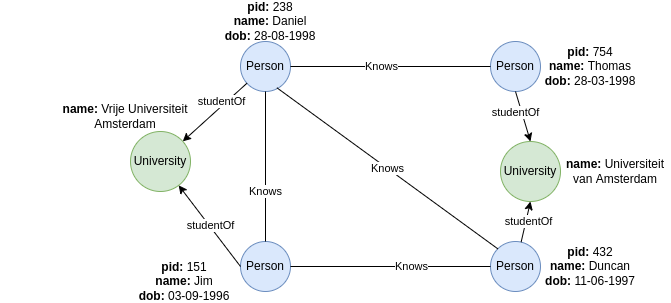
\includegraphics[width=\linewidth]{figures/friend-graph.png}
  \caption{Graph of friend network and where they study.}
  \label{fig:graph-friend}
\end{figure}


To match a pattern to this graph in SQL/PGQ, the \textcolor{blue}{\texttt{MATCH}} syntax can be used~\cite{Deutsch2021}, as can be seen in Listing~\ref{app:sqlpgqmatchnode}. 
% Matching graph patterns forms the core for many graph query languages and are sometimes also referred to as Regular Path Queries (RPQs)~\cite{Deutsch2021}.
For example, the following selects the name and date of birth from persons from the graph in Figure~\ref{fig:graph-friend} whose name is equal to 'Daniel': 
\begin{lstlisting}[caption=Pattern matching all nodes with the property name Daniel, label=app:sqlpgqmatchnode] 
SELECT p.name, p.dob
FROM Person GRAPH_TABLE (
    MATCH ( a:Person WHERE a.name = 'Daniel' )
    COLUMNS (
        a.name,
        a.dob )
    ) p
\end{lstlisting}

Matching such a simple graph pattern is also relatively straightforward in plain SQL, however, it could be argued that the SQL/PGQ syntax feels more natural to write than the plain SQL one, since it is closer to how the human mind tends to interpret the world regarding objects and their connections~\cite{benkler2008collective}. 
As can be seen in Listing~\ref{app:sqlpgqmatchnode}, we use the () notation to address a node. Addressing an edge can be done by using \texttt{[]}. To indicate that an edge is pointing from source to destination we use \texttt{(source)-[edge pattern]->(destination)}. This ASCII-art style is inspired by the syntax of Cypher, one of the most widely used graph query language~\cite{cypher-popularity}. 

A more complex graph pattern, involving both nodes and undirected edges could look like the following: 
\begin{lstlisting}[caption=Pattern matching using nodes and edges, label=app:sqlpgqmatchnodeedge] 
MATCH ( a:Person WHERE a.name = 'Daniel' )-[ e:knows ]-( b:Person )-[ f:studentOf ]-( c:University ) 
\end{lstlisting}

This statement would extract all patterns that match node $a$ being a Person with the name Daniel, who knows a Person who is a studentOf a University. Within every node or edge, we can filter the possibilities by adding a \textcolor{blue}{\texttt{WHERE}} statement, as can be seen in Listing~\ref{app:sqlpgqmatchnodeedge}.

One of the features of SQL/PGQ will be the ability to match a single edge pattern or a parenthesized path pattern for an arbitrary length~\cite{Deutsch2021}. 
An example where we want to find paths of length 2 to 5 of \textit{knows} edges: 
\begin{lstlisting}[caption=Path length of 2 to 5 knows edges, label=app:sqlpgqmatch25knows] 
MATCH ( a:Person )-[ e:knows ]->{2,5}( b:Person )
\end{lstlisting}
Finding such a path in plain SQL is significantly more difficult~\cite{oracle-sql-example}. 
SQL/PGQ is not limited to quantifying the upper-bound of the path length in such a path finding query. 
Similar to regular expressions, it is possible to use the Kleene star (*) operator, to indicate that the pattern can occur 0 or more times. 
Additionally, matching the pattern 1 or more times is possible using the Kleene plus (+) symbol.
The following is an example of a pattern using the Kleene star operator: 
\begin{lstlisting}[caption=Path length of arbitrarily many knows edges, label=app:sqlpgqmatchkleene] 
MATCH ( a:Person )-[ e:knows ]->*( b:Person )
\end{lstlisting}

Another addition in SQL/PGQ will be the ability to return the path corresponding to a query.
Alongside returning every path that adheres to a given pattern, it will be possible to return the cheapest or shortest path. 
The cheapest path will return the path in which the total weight of the edges along the path are the lowest.
The shortest path returns the path containing the least amount of hops from the starting node to the end node.
In case the graph is unweighted, cheapest and shortest path will provide equivalent results, since the weight of any edge will be equal to 1.
% A matching pattern containing the cheapest path will be of the format: 
% \begin{lstlisting}[caption=Matching the cheapest path, label=app:sqlpgqmatchcheapest] 
% MATCH CHEAPEST < pattern >
% \end{lstlisting}

% In the GQL manifesto~\cite{gqlmanifesto}, Green highlighted three similar query languages (Cypher, G-CORE, and PGQL) that coexisted, which he believed should be standardized into one. 
% Following will be a more in-depth look at those three languages, and how they differ from each other. 

% First, one of the most widely used query languages, Cypher~\cite{cypher-popularity} which was developed by Neo4j. 
% % It is currently an open-source project maintained by the openCypher Implementers Group~\cite{Francis2018}. 
% % One of the goals of providing an open-source language was to stimulate the transition from the openCypher implementation to the GQL standard and prevent a form of vendor lock-in~\cite{opencypher}. 
% A key feature of Cypher is the ASCII-art syntax for pattern matching. Additionally, if a vertex or edge with a specific label should be matched, one would write \texttt{(a:Account)-[r:Transfer]->{2..*}(b:Account)}. Here vertices (a) and (b) have the label 'Account', and the path is a directed edge as indicated by the arrow which has the label 'Transfer'.
% This intuitive syntax makes it an easy language to pick up~\cite{cypher-popularity}. 
% However, the query language has several shortcomings, namely the lack of regular path queries (RPQs) and graph construction~\cite{10.1145/2960414.2960421}. Regular path queries are recursive queries that define a path using regular expressions.

% The second graph query language is PGQL, which was created by Oracle Labs.
% PGQL follows a more SQL-like syntax and functionalities and provides functionalities for RPQs and graph construction.
% A PGQL query consists of three mandatory clauses \textit{SELECT}, \textit{FROM}, and \textit{WHERE} which can be followed by any of the optional clauses \textit{ORDER BY}, \textit{GROUP BY}, and \textit{LIMIT}. 
% The PGQL developers argue that the SQL-like syntax for PGQL allows existing SQL users to switch easily between the two languages~\cite{10.1145/2960414.2960421}. 

% The final graph query language from which inspiration was taken was G-CORE~\cite{DBLP:conf/sigmod/AnglesABBFGLPPS18}. The language was developed by the LDBC Graph Query Language Task Force~\cite{ldbc} which consists of members from industry and academia. The task force used the core of current existing graph languages as a base to develop G-CORE. They provide a formal definition of G-CORE to help correct the development of the language~\cite{gcoreparser}. The main deviation of G-CORE compared to other languages is how it treats paths as first-class citizens. It essentially means that paths become just as important as nodes and edges, allowing users to use paths in their queries. 

\subsection{Graph traversal algorithms}
\subsubsection{Multi-Source Breadth-First Search (MS-BFS)}
In order to compute the shortest path of unweighted graphs, the batched variant of the MS-BFS algorithm developed by Then et al.~\cite{10.14778/2735496.2735507} can be used. The pseudo-code of the algorithm is provided in Algorithm~\ref{alg:msbfs}. 
The algorithm is an example of a bulk algorithm that fits well in the vectorized execution engine of DuckDB~\cite{keynote-boncz-edbt-icdt-2022}. 
It is able to run multiple BFSs concurrently on the same graph in a single CPU core. 
Furthermore, it can make use of Single Instruction Multiple Data (SIMD) instructions, such as AVX-512~\cite{avx512}, that are available in modern CPUs. 
This lets us handle 512 BFS steps in one CPU cycle, further increasing the efficiency in CPU usage. 
Additionally, it has the ability to scale up as the number of CPU cores increases. Since there are no dependencies between the various BFSs, they can be divided over multiple cores. 
It makes use of the small-world property~\cite{smallworld} that occurs when the diameter of a graph is small in comparison to the total number of nodes.
This means that each BFS discovers most vertices in a few iterations, and concurrent BFSs have a high chance of overlapping sets of discovered edges in the same iteration. 
This allows access to be shared among the multiple BFSs and reduce the chance of cache misses, reducing the overall computation time~\cite{10.14778/2735496.2735507}.


\begin{algorithm}
\caption{MS-BFS}
\label{alg:msbfs}
\begin{algorithmic}[2]
    \State \textbf{Input:} $G,\mathbbm{B},s$
    \State $seen_{s_i} \leftarrow \{b_i\} \:for \: all \: b_i \in \mathbbm{B}$
    \State $visit \leftarrow \bigcup_{b_i \in \mathbbm{B}}\{(s_i,\{b_i\})\}$
    \State $visitNext \leftarrow \varnothing$
    
    \While {$visit \neq \varnothing$}
        \For {\textbf{each} $v \: \textbf{in} \: visit$}
            \State $\mathbbm{B}'_v \leftarrow \varnothing$
            \For {\textbf{each} $(v', \mathbbm{B}') \in visit \: \textbf{where} \: v' = v$}
                \State $\mathbbm{B}'_v \leftarrow \mathbbm{B}'_v \cup \mathbbm{B}'$
            \EndFor
            \For {\textbf{each} $n \in neighbours_v$}
                \State $\mathbbm{D} \leftarrow \mathbbm{B}'_v \setminus seen_n$
                \If {$\mathbbm{D} \neq \varnothing$}
                    \State $visitNext \leftarrow visitNext \cup \{(n,\mathbbm{D})\}$
                    \State $seen_n \leftarrow seen_n \cup \mathbbm{D}$
                    \State Do BFS computation on $n$
                \EndIf
            \EndFor
        \EndFor
        \State $visit \leftarrow visitNext$
        \State $visitNext \leftarrow \varnothing$
    \EndWhile   
\end{algorithmic}
\end{algorithm}


\subsubsection{Cheapest path}
To find a cheapest path in weighted graphs either the Dijkstra or Bellman-Ford algorithms can be used. The Dijkstra algorithm has a worst-case time complexity of $\mathcal{O}(|E|+|V|\log|V|)$~\cite{10.1145/28869.28874}, which is better than Bellman-Ford's worst-case time complexity of $\mathcal{O}(|V|\cdot|E|)$~\cite{bannister2011randomized}.
However, the expected runtime of Bellman-Ford is $O(|E|)$ in large dense graphs with low diameter~\cite{Yen1970AnAF}.
Then et al.~\cite{DBLP:journals/dbsk/ThenGKN17} propose a Batched Bellman-Ford-based algorithm, shown in Algorithm~\ref{alg:batched-bellman-ford}, to find the shortest distance between two nodes in a graph.
This algorithm can make use of SIMD instructions to increase the CPU usage efficiency, which is not possible with the standard Bellman-Ford algorithm~\cite{bellman1958routing}, which is shown in Algorithm~\ref{alg:bellman-ford}. 

\begin{algorithm}
\caption{Bellman-Ford}
\label{alg:bellman-ford}
\begin{algorithmic}[2]
    \State Initialize-Single-Source(G,s)
    \For {$i \leftarrow 1$ to $|V[G]| - 1$}
        \For {\textbf{each} edge $(u,v) \in E[G]$}
            \State Relax(u, v, w)
        \EndFor
    \EndFor
    \For {\textbf{each} $edge (u,v) \in E[G]$}
        \If {$d[v] > d[u] + w(u, v)$}
            \State Return False
        \EndIf
    \EndFor
    
 
\end{algorithmic}
\end{algorithm}

\begin{algorithm}
\caption{Directed batched Bellman-Ford-based algorithm}
\label{alg:batched-bellman-ford}
\begin{algorithmic}[2]
    \State \textbf{Input: WeightedGraph G, Array<Vertex>} sources
    \State \textbf{Output: VertexProperty<BatchVar<double>\>>} dists
    
    \State \textbf{VertexProperty<BatchVar<bool>\>>} modified = false
    \State dists = Infinite
    
    \For {i=1..sources.length}
        \State \textbf{Node} v = sources[i]
        \State dists[v][i] = 0
        \State modified[v][i] = true
    \EndFor
    
    \State \textbf{bool} changed = true
    \While{changed}
        \State changed = false
        \For{\textbf{each} v in G.vertices}
            \If{not modified[v].empty()}
                \For{\textbf{each} v in G.neighbours(v)}
                    \State double weight = edgeWeight(v,n)
                    \For{\textbf{each} i in modified[v]}
                        \State \textbf{double} newDist = min(dists[n][i], dists[v][i] + weight)
                        \If {newDist != dists[n][i]}
                            \State dists[n][i] = newDist
                            \State modified[n][i] = true
                            \State changed = true
                        \EndIf
                    \EndFor
                \EndFor
            \EndIf
        \EndFor
    \EndWhile
    
 
\end{algorithmic}
\end{algorithm}


\subsection{DuckDB}
DuckDB is a database management system specialized in OLAP workloads~\cite{DBLP:conf/sigmod/RaasveldtM19}.
This means that the system is optimized more towards analytical queries, touching large data volumes using joins and aggregations.
Just like SQLite, DuckDB is an in-process system, though SQLite is specialized in OLTP workloads.

DuckDB consists of a number of components: Parser, logical planner, optimizer, physical planner, and execution engine. 
The system can be accessed through a C/C++ API, as well as a SQLite compatibility layer. 
The SQL parser is based on the PostgreSQL SQL parser~\cite{DBLP:conf/sigmod/RaasveldtM19}.
The logical planner consists of a binder and a plan generator.
The binder is responsible for the expressions from the query related to anything containing a schema such as tables and views and retrieves the required columns and data types. 
The plan generator then creates a tree of basic logical query operators from the retrieved parse tree. 
Once the logical planner is done, the optimizer is used to optimize the logical plan. 
This will result in an optimized logical plan which is given to the physical planner where it is turned into a physical plan.
The physical plan consists of operators, where each operator implements one step of the plan. 
An example of a unary operator is the \textit{scan}, which scans a table and brings each tuple of a relation into main memory~\cite{DBLP:books/daglib/0020812}.
A join operator that makes use of two tables is an example of a binary operator.

These operators are split up into pipelines, which determines the order of operation execution.
A query can consist of one or more pipelines, some of which contain a dependency on another pipeline. 
A pipeline with a dependency is for example, one containing a join operator. 
The start of a pipeline is referred to as a source and the end is referred to as the sink, which is where all the data is collected (materialized).
Only sink operators, such as sorting, building a hash table, and hash aggregation need to see all the data before they can proceed. All other operators do not need to materialize all data before proceeding. 
In the case of binary operators there are always two pipelines, one that builds the hash table, and one that probes this hash table. Both pipelines contain a source and a sink, and since the probing is a non-materializing operation it can be scheduled in the middle of a pipeline. 


With every join, a hash table needs to be built on which the join can be performed and the operator needs to wait for the entire hash table to be built.  
Only then can the join be correctly executed.
In the same vein, another pipeline might require the outcome of this join before it can be executed, creating a chain of dependencies.

DuckDB makes use of hash tables to perform join operations\footnote{Whenever the ids of the smaller table are dense, meaning the maximum id is not much larger than the size of the table, an array is used instead, eliminating the need to build a hash table. This is referred to as a perfect join~\cite{DBLP:conf/sigmod/AbadiMH08}.}. 
Cardinality estimation is performed to asses which of the two tables is the smaller one. These estimations can be wrong, so it is not guaranteed that the smallest table is always used. 



This smallest table is then used to build a hash table from, this is also referred to as the \textit{sink} or the build side. 
The other, larger, table is then used to probe the hash table, looking for matching entries, this is referred to as the \textit{source} or the probe side.
Whenever the two tables are of equal size, a random one of the two is chosen to be the sink. 

% After finalizing the physical plan, a pipeline is constructed in which the order of operator execution is determined.


The execution engine of DuckDB is vectorized~\cite{DBLP:conf/sigmod/RaasveldtM19}. The use of vectors is more CPU efficient than the more common tuple-at-a-time execution found in other DBMSs~\cite{DBLP:conf/cidr/BonczZN05}. 
ACID-compliance (\textbf{A}tomic, \textbf{C}onsistent, \textbf{I}solated, and \textbf{D}urable) in DuckDB is provided by Multi-Version Concurrency Control~\cite{DBLP:conf/sigmod/RaasveldtM19}.
To allow for persistent storage, DuckDB uses the DataBlocks storage layout, which is read-optimized~\cite{DBLP:conf/sigmod/RaasveldtM19}.
A useful feature of DuckDB is the allowance of extension modules, also referred to as Scalar user-defined functions (UDFs).
These Scalar UDFs are as fast as the built-in functions of DuckDB due to the vectorized query processing, meaning that the parallelization of the UDF is handled by DuckDB. 


\subsection{Current state of SQL/PGQ in DuckDB}\label{sec:sofar}
This thesis will continue upon the work done by Singh et al.~\cite{sqlpgq-duckdb}. They identified several challenges that needed to be addressed. 
DuckDB is primarily intended for tabular workloads and wants to limit its core features to those required for the the tabular types of workloads.
One of the first challenges to be tackled was successfully parsing SQL/PGQ queries. 
The SQL/PGQ queries are transformed into plain SQL queries, for example, see Listing~\ref{app:sqlpgqquery2} and Listing~\ref{app:sqlpgqquerykleene}. 
It can be observed that Listing~\ref{app:sqlpgqquerykleene} contains a Kleene star, making it more difficult to transform into a plain SQL query. 
Since SQL/PGQ contains new statements (e.g. GRAPH, LABEL, PROPERTIES, see Listing~\ref{app:sqlpgqfriendnetwork}), these had to be added to the parser of DuckDB. 
Therefore, minimal changes to the parser and transformer were made to allow correct parsing of SQL/PGQ queries.  
Another consequence of limiting the core features was the decision to implement the new operators, such as the batched MS-BFS algorithm~\cite{10.14778/2735496.2735507}, as UDFs. 
With MS-BFS it is possible to compute the reachability of any number of nodes given one or more source nodes. 
DuckDB handles the parallelization for Scalar UDFs using the morsel-driven method~\cite{duckdb-morsel-driven}, which helps when scaling the batched MS-BFS algorithm.
Another benefit of implementing these operators as Scalar UDFs instead of expressions is the fact that little to no changes have to be made to the internals of DuckDB. 
For example, to implement reachability, no further changes needed to be made to the parser and no new logical and physical operators had to be introduced. 

Another challenge Singh et al. looked at was the access patterns. 
Typically, a pointer-based data structure can be used for $O(1)$ lookup. 
In this case, every node contains a mini-index to all nearby nodes~\cite{indexfreeadjacency}. 
However, this becomes inefficient in the case of multiple traversals due to poor memory locality. 
An alternative is to make use of a Compressed Sparse Row (CSR) data structure.
With this data structure, the rowids of both the vertex and edge tables are condensed into integers in the range  $[0, |V|)$ and $[0, |E|)$.  
Most importantly are the edge tables, which are usually much larger, leading to a higher chance of poor memory locality. 
Thus, Singh et al. created a UDF to create such CSR-like data structures, which are then used during the execution of the MS-BFS UDF.
A weighted graph is represented in Figure~\ref{fig:weightedgraph}.
The rows in the table represent the source vertices, while the columns represent the destination vertices. 
Vertices that share an edge contain a weight, ranging between $[0, 1)$ in this example in their respective cell. 
For example, the edge from vertex 1 to vertex 2 has a weight of $.3$.
Figure~\ref{fig:csrweightedgraph} shows the CSR representation for the graph in Figure~\ref{fig:weightedgraph}. 
The row pointers point to the index of the first column for which there is an edge going from the row index to the column index. 
For example, in Figure~\ref{fig:weightedgraph} we observe the first edge from row 1 goes to column 2. 
For row 4, the first edge goes to column 1, therefore, the row pointer 4 goes to column index 1. 
The offset between two row pointers can be used to determine the number of edges for a row.
The value corresponding to the edge can be found in a separate array using the same index as the column index.
This condenses the matrix-like data structure into regular arrays, improving the memory locality. 

\begin{figure}
  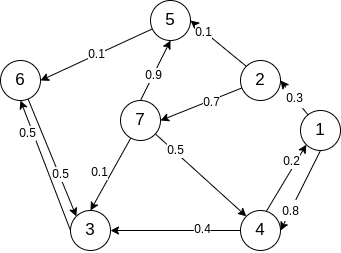
\includegraphics[width=0.6\linewidth]{figures/CSR diagrams.drawio.png}
  \caption{An example of a weighted graph}
  \label{fig:weightedgraph}
\end{figure}


\begin{figure}
  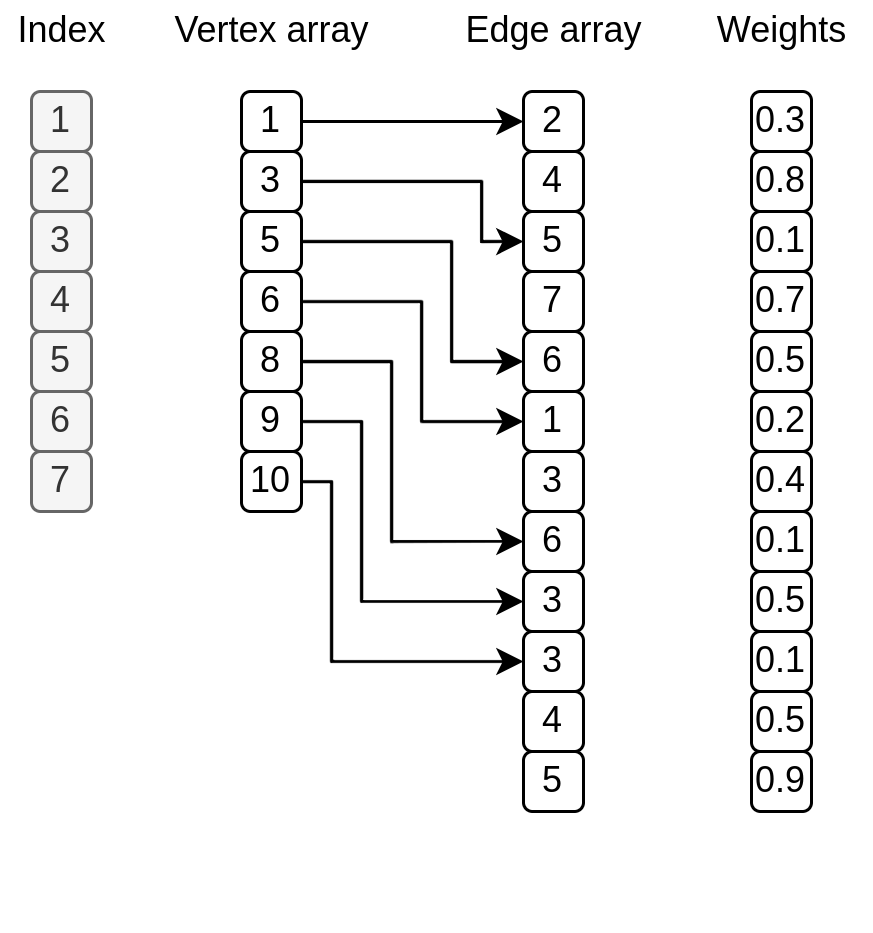
\includegraphics[width=0.6\linewidth]{figures/csr-representation.png}
  \caption{CSR representation of graph in Figure~\ref{fig:weightedgraph}}
  \label{fig:csrweightedgraph}
\end{figure}

% \begin{table}[!ht]
%     \centering
%     \begin{tabular}{|l|l|l|l|}
%     \hline
%         rowid & pid & name & dob \\ \hline
%         0 & 238 & Daniel & 28-08-1998 \\ \hline
%         1 & 151 & Jim & 03-09-1996 \\ \hline
%         2 & 754 & Thomas & 28-03-1998 \\ \hline
%         3 & 432 & Duncan & 11-06-1997 \\ \hline
%     \end{tabular}
    
%     \caption{Vertex table Person}
%     \label{tab:vperson}
%     \quad
%     \begin{tabular}{|l|l|l|}
%     \hline
%         rowid & p1\_id & p2\_id \\ \hline
%         0 & 238 & 151 \\ \hline
%         1 & 238 & 754 \\ \hline
%         2 & 238 & 432 \\ \hline
%         3 & 151 & 238 \\ \hline
%         4 & 151 & 432 \\ \hline
%         5 & 754 & 238 \\ \hline
%         6 & 432 & 238 \\ \hline
%         7 & 432 & 151 \\ \hline
%     \end{tabular}
%     \caption{Edge table knows}
%     \label{tab:eknows}

% \end{table}

% \begin{table}[!ht]
%     \centering
%     \begin{tabular}{|l|l|}
%     \hline
%         p1\_id & p2\_id \\ \hline
%         238 & 151 \\ \hline
%         238 & 754 \\ \hline
%         238 & 432 \\ \hline
%         151 & 238 \\ \hline
%         151 & 432 \\ \hline
%         754 & 238 \\ \hline
%         432 & 238 \\ \hline
%         432 & 151 \\ \hline
%     \end{tabular}
%     \caption{Edge table knows}
%     \label{tab:eknows}
% \end{table}

% \begin{table}[!ht]
%     \centering
%     \begin{tabular}{|l|l|}
%     \hline
%         id & name \\ \hline
%         1 & Vrije Universiteit Amsterdam \\ \hline
%         2 & Universiteit van Amsterdam \\ \hline
%     \end{tabular}
%     \caption{Vertex table University}
%     \label{tab:vuniversity}
% \end{table}

% \begin{table}[!ht]
%     \centering
%     \begin{tabular}{|l|l|}
%     \hline
%         university\_id & person\_id \\ \hline
%         1 & 1 \\ \hline
%         1 & 2 \\ \hline
%         2 & 3 \\ \hline
%         2 & 4 \\ \hline
%     \end{tabular}
%     \caption{Edge table studentOf}
%     \label{tab:estudentOf}
% \end{table}